\documentclass[11pt,letterpaper]{article}
\usepackage[utf8]{inputenc} %Codificacion del texto (ISO Latin1 encoding)

\usepackage{fancyhdr} %Permite acomodar a tu gusto la parte de arriba y
% abajo del documento
\usepackage[spanish]{babel} %Permite definir el idioma del dcumento
\usepackage{graphicx} %Permite exportar imagenes en formato eps
\usepackage{url} %Tipo de fuente para correos y paginas
\usepackage{pgf}
\usepackage{fleqn}
\usepackage{amssymb}
\usepackage{fancyvrb}
\usepackage{sectsty}
\usepackage{makeidx}
\usepackage{colortbl} %Permite colocar colores a las tablas
\usepackage{booktabs}
\definecolor{red}{rgb}{1,0,0}
%%%%%%%%%%
%Margenes%
%%%%%%%%%%
\parskip 1mm %Espacio entre parrafos

\setlength{\topmargin}{0pt}

\oddsidemargin	0.5cm  % Ancho Letter 21,59cm
\evensidemargin 0.5cm  % Alto  Letter 27,81cm
\textwidth	15.5cm
\textheight	21.0cm
\headsep	4 mm
\parindent	0.5cm
%%%%%%%%%%%%%%%%%%%%%%
%Estilo del documento%
%%%%%%%%%%%%%%%%%%%%%%
\pagestyle{fancyplain}

%%%%%%%%%%%%%%%%%%%%%%%%%%%%%%%%%%%%%%%%%%%
%Fancyheadings. Top y Bottom del documento%
%%%%%%%%%%%%%%%%%%%%%%%%%%%%%%%%%%%%%%%%%%%
% Recuerde que en este documento la portada del documento no posee
% numeracion, pero de igual manera llamaremos a esa primera pagina la numero
% 1, y la que viene la dos. Esto es para tener una idea de las que
% llamaremos pares e impares
\lhead{Estadistica Computacional} %Parte superior izquierda
\rhead{\bf \it Resumen C1 2008-2} %Parte superior derecha
\lfoot{\it EB/RF/GZ/CM/\LaTeX} %Parte inferior izquierda. \thepage indica
% el numero de pagina
\cfoot{} %Parte inferior central
\rfoot{\bf \thepage} %Parte inferior derecha
\renewcommand{\footrulewidth}{0.4pt} %Linea de separacion inferior

% Challa

\newtheorem{theorem}{Theorem}
\newtheorem{acknowledgement}[theorem]{Acknowledgement}
\newtheorem{algorithm}[theorem]{Algorithm}
\newtheorem{axiom}[theorem]{Axiom}
\newtheorem{case}[theorem]{Case}
\newtheorem{claim}[theorem]{Claim}
\newtheorem{conclusion}[theorem]{Conclusion}
\newtheorem{condition}[theorem]{Condition}
\newtheorem{conjecture}[theorem]{Conjecture}
\newtheorem{corollary}[theorem]{Corollary}
\newtheorem{criterion}[theorem]{Criterion}
\newtheorem{definition}[theorem]{Definition}
\newtheorem{example}[theorem]{Example}
\newtheorem{exercise}[theorem]{Exercise}
\newtheorem{lemma}[theorem]{Lemma}
\newtheorem{notation}[theorem]{Notation}
\newtheorem{problem}[theorem]{Problem}
\newtheorem{proposition}[theorem]{Proposition}
\newtheorem{remark}[theorem]{Remark}
\newtheorem{solution}[theorem]{Solution}
\newtheorem{summary}[theorem]{Summary}
\newenvironment{proof}[1][Proof]{\noindent\textbf{#1.} }{\ \rule{0.5em}{0.5em}}

\newcommand{\primaria}[1]{
	\textbf{\underline{#1}}
}

\newcommand{\foranea}[1]{
	\textbf{\textsl{#1}}
}

\newcommand{\primyfor}[1]{
	\underline{\foranea{#1}}
}

\makeatletter
\newcommand\subsubsubsection{\@startsection {paragraph}{1}{\z@}%
                                   {-3.5ex \@plus -1ex \@minus -.2ex}%
                                   {1.5ex \@plus.2ex}%
                                   {\normalfont\bfseries}}
\newcommand\subsubsubsubsection{\@startsection {subparagraph}{1}{\z@}%
                                   {-3.5ex \@plus -1ex \@minus -.2ex}%
                                   {1.5ex \@plus.2ex}%
                                   {\normalfont\bfseries}}


\makeatother

%\makeindex
%%%%%%%%%%%%%%%%%%%%%%%%%%%%%%%%%%%%%%%%%%%%%%%%%%%%%%%%%%%%%%%%%%%
%%%%%%%%%%%%%%%%%%%% Aqui empieza el documento %%%%%%%%%%%%%%%%%%%%
%%%%%%%%%%%%%%%%%%%%%%%%%%%%%%%%%%%%%%%%%%%%%%%%%%%%%%%%%%%%%%%%%%%

\begin{document}

%%%%%%%%%%%%%%%%%%%%%%%%%%
%Definicion de la portada%
%%%%%%%%%%%%%%%%%%%%%%%%%%
\begin{titlepage}
    \begin{center}
	\begin{tabular}{ccc}
	    %\epsfig{file=escudo-utfsm.eps, height=1.6cm}
	      
\includegraphics[height=1.6cm]{images/logoUTFSM}
	    & %Escudo de la Universidad Santa Maria
	    \hspace{0.2cm}
	    \begin{tabular}{c}
		Universidad Técnica Federico Santa María \\ \hline
		\hspace{8.0cm}
		\vspace{1.2cm}
	    \end{tabular}
	    \hspace{0.2cm}
	    &
	   % \epsfig{file=logo_DI.eps, height=1.6cm} %Logo del DI
            
\includegraphics[height=1.6cm]{images/logoDI}
	\end{tabular}

	\vspace{2.5cm}
	%Titulo del Documento
	    \begin{tabular}{c}
		\Huge{\textbf{Tarea 2}}\\\\\\\\\\\\\\
		\LARGE{\textbf{``Sistema de Gesti\'on de Clientes VIP''}}\\\\
		\LARGE{\sc{Fundamentos de Ingenier\'ia}}\\
		\LARGE{\sc{de Software}}
	    \end{tabular}

	\vspace{2.5cm}
%	\begin{tabular}{c}
	\begin{center}
%	     \pgfimage[height=1.8cm]{images/now}
	%    \Huge{\emph{Now!}}
%	\end{tabular}
	\end{center}
	
        \vspace{1.5cm}

	%Nombre del (o los) autor(es)
	\begin{tabular}{lr}
            \begin{tabular}{c}
	        \large{Rodrigo Fern\'andez - 2673002-3}\\
		\large{\url{rfernand@inf.utfsm.cl}}
	    \end{tabular}
	&
	   \begin{tabular}{c}
         	\large{Cristi\'an Maureira - 2673030-9}\\ 
		\large{\url{cmaureir@inf.utfsm.cl}}
	   \end{tabular}
	\end{tabular}
        \vspace{3.5cm}\\
	%Fecha
		\large{\sc{Valpara\'iso, Octubre 2008.}}
    \end{center}
\end{titlepage}


\section{Muestreo y Presentaci\'on de los Datos}
\label{sec:cap1}
\begin{itemize}
\item[\textbf{1.8}] \emph{?`Cu\'ales de las siguientes instrucciones deber\'ia
ser priviligiada?}\\
R:
	\begin{itemize}
		\item \textcolor{red}{Set value of timer}
		\item Read the clock
		\item \textcolor{red}{Clear memory}
		\item Issue a trap instruction
		\item \textcolor{red}{Turn off interrupts}
		\item \textcolor{red}{Modify entries in device-status table}
		\item Switch from user to kernel mode
		\item \textcolor{red}{Access I/O device}
	\end{itemize}

\item[\textbf{1.13}] \emph{En un entorno de multiprogramaci\'on y tiempo
compartido, varios usuarios comparten el sistema simult\'aneamente.Esta
situaci\'on puede resultar en varios problemas de seguridad}\\
	\begin{itemize}
		\item ?`Cu\'ales son los dos problemas?\\
R:\\
 El robo o copiado de la informaci\'on o programas de un usuario y el usar los recursos del sistema (CPU, memory,disk space, peripherals) sin un sistema de cuentas apropiados.
 Por ello, es necesario que exista mecanismos de seguridad, para evitar la
espera permanente de un proceso, y se debe proveer de mecanismos para la
sincronizaci\'on de procesos a si como su debido sistema de permisos. 

		\item ?`Podemos asegurar el mismo grado de seguridad en una m\'aquina de tiempo compartido, como en una m\'aquina dedicada? Explicar la respuesta\\
R:\\
 Los sistemas dedicados, poseen un grado mayor de seguridad, ya que es limitado para los usuarios.
	\end{itemize}

\item[\textbf{1.17}] \emph{Describa las diferencias entre el multiprocesamiento sim\'etrico y asim\'etrico. ?`Cu\'ales son las 3 ventajas y 1 desventaja del sistemas multiprocesos?}\\
R:\\
	En el multiprocesamiento simetrico no existe relaci\'on entre los procesadores, todos van a la par. En cambio, en el asimetrico, la relaci\'on entre los procesadores es del tipo maestro-esclavo.\\
	Por otro lado, en el simetrico se deben manetener mecanismos de seguridad que administren el procesamiento de los jobs (que no se elija el mismo, que no se extravi\'en, sincronizar los recursos entre ambos procesadores).\\
	 En el asimetrico, si falla el procesador maestro, falla todo el sistema.\\\\
	\begin{itemize}
	\item Ventajas Multiprocesamiento:
	\begin{enumerate}
		\item Incrementa rendimiento, eficiencia, mayores procesos corriendo simultaneamente.
		\item Economia de Escala.
		\item Toleracia a fallas
	\end{enumerate}
	\item Desventaja:
	\begin{enumerate}
		\item Mas complejo.
	\end{enumerate}
	\end{itemize}

\item[\textbf{1.22}] \emph{?`Cu\'al es el prop\'osito de las
interrupciones??`Cu\'ales son las diferencias entre una ``trap'' y una
``interrupci\'on''??`Pueden las ``traps'' ser generadas intencionalmente por
un programa de usuario?Si es asi, ?`Para qu\'e proposito?}\\
R:\\
		Las iterrupciones son los mensajes que los dispositivos envian al SO para adquirir el control de la CPU.\\
		Las trap o excepci\'on son interrupciones generadas a nivel de software cuando sucede algun tipo de error (ej: division por 0, loop infinito, procesos modificandose entre si o al SO), para terminar intencionalmente la ejecuci\'on de un proceso.\\

\item[\textbf{1.23}] \emph{DMA es usado por dispositivos I/O de alta velocidad
para evitar el aumento de la carga de la ejecuci\'on de la CPU}\\
	\begin{itemize}
		\item ?`C\'omo funciona la interfaz de CPU con el dispositivo para coordinar la transferencia?\\
R:\\
			A traves de dos posibles metodos:
			\begin{enumerate}
				\item Metodo simple: Rutina gen\'erica invoca a la espec\'ifica (muy lento).
				\item Tener una tabla en la cual se almacena una lista de punteros a las rutinas de interruci\'on (se llama a la rutina de interrupci\'on de forma indirecta a trav\'es de la tabla). Dicha matriz se indexa con un n\'umero de dispositivo unico. (Windows y UNIX)
			\end{enumerate}
		\item ?`C\'omo sabe la CPU cuando las operaciones de  memoria se completan?\\
R:
			Porque los dispositivos envian una interrupci\'on avisando que se completo la trasmici\'on.

		\item La CPU esta permitida de ejecutar otros programas mientras que el controlador DMA esta tranferiendo datos.?`Puede \'este proceso interferir con la execuci\'on de los programas de usuario? Si es as\'i, describir que formas de interferencia son causados.
R:\\
			No interfiere, ya que la transferencia de datos no utiliza cpu, ni ciclos de m\'aquina.% Pero aun asi, el proceso puede interferir si intenta modificar algun dato que este siendo transferido. Esto se evita bloqueando las zonas que esten siendo utilizadas.
	\end{itemize}

\item[\textbf{1.24}] \emph{Algunos sistemas computacionales no proveen un modo
de operaci\'on privilegiado en hardware.?`Es posible contruir un SO seguro
para estos sistemas computacionales?} Dar argumentos en caso que sea posible o
no\\
R:\\
No es posible construir un SO seguro para este sistema inform\'atico, ya que se requiere protecci\'on para ciertos accesos a hardware por parte del usuario.

\item[\textbf{1.30}] \emph{Definir las propiedades escenciales de los
siguientes tipos de SO}\\
R:
	\begin{itemize}
		\item Batch
		\begin{enumerate}
			\item Ejecuci\'on de procesos sin interacci\'on con humanos.
			\item Toda la informacion de entrada esta definida en scripts o en parametros de una linea de comandos.
			\item Rapido y eficiente gracias a que no esta constantemente interactuando con el usuario.
		\end{enumerate}	
		\item Interactive
		\item Time sharing	
		\begin{enumerate}
			\item	Tambien llamada multi-tarea, es una extensi\'on logica en la cual la CPU cambia entre jobs frecuentemente de tal forma que los usuarios puedan interactuar con cada job mientras este corre.
			\item A lo anterior se le llama computaci\'on interactiva.
			\item Tiempo de respuesta: menor a 1 segundo.
			\item Procesos: Cada usuario tiene al menos un programa ejecutandose en memoria.
			\item CPU Scheduling.
			\item Swapping de procesos si estos no caben enteros en la memoria.
			\item Uso de memoria virtual para la ejecucion de procesos que no estan completamente en la memoria.
		\end{enumerate}
		\item Real time
		\begin{enumerate}
			\item Sistema operativo multi-tarea dirigido a aplicaciones de tiempo real. 
			\item Latencia m\'inimal de las interrupciones y del cambio de threads.
			\item Priority scheduling: Cambia de tarea solo cuando surge un evento de mayor prioridad.
			\item Time-sharing: Basicamente, usa round robin. 
		\end{enumerate}
		\item Network
		\begin{enumerate}
			\item Controla la red, sus traficos de mensajes y sus colas de acceso. Administra los recursos de la red y provee seguridad a la misma. 
			\item Soporte basico de puertos de hardware
			\item Seguridad: Restricciones de autentificacion, autorizacion y login (controles de acceso).
			\item Servicios de nombre y de directorios. 
			\item De acceso remoto, y administracion a traves de la red.
			\item Tolerante a los fallos y posee una alta disponibilidad. 
		\end{enumerate}
		\item Parallel
		\begin{enumerate}
			\item De arquitectura mas compleja que los de programacion secuencial.
			\item Debe introducir controles para evitar problemas o bugs gracias al uso concurrente de los recursos.. 
			\item Mas vel\'oz, y su velocidad es regida por la ley de Amdahl's 
			\item La mayor barrera para tener un buen rendimiento es la obtencion de un buen sistema de comunicaci\'on y sincronizaci\'on de las diferentes sub-procesos. 
		\end{enumerate}
		\item Distributed
		\begin{enumerate}
			\item Un tipo de computaci\'on paralela. 
			\item Distribuye la memoria del sistema conectando los elementos de procesamientos a traves de una red.
			\item Gran escalabilidad.
			\item Parecido al Network SO, solo que la plataforma en la cual corre debe poseer una gran configuraci\'on y mas capacidad de RAM, altas velocidades del Procesador.
		\end{enumerate}
		\item Clustered
		\begin{enumerate}
			\item Ejecuci\'on Remota Trasparente:\\ Las aplicaciones deben ser ignorar el hecho de que un proceso puede estar corriendo en un nodo propio o remoto 
			\item Balance de Carga: \\ Debe implementar un inteligente mecanismo de colocaci\'on de procesos.
 			\item Compatibilidad Binaria:\\ Debe proveer una ejecuci\'on remota trasparente, balanceo de carga y otras caracter\'isticas, sin requerir modificar aplicaciones ni volver a generar enlaces.
 			\item Alta disponibilidad:\\ Si un nodo falla, el sistema puede continuar operando.
 			\item Portable:\\ Tiene que poder serlo!
		\end{enumerate}
		\item Handheld
		\begin{enumerate}
			\item Como Palm OS, Android y relativos.
		\end{enumerate}
	\end{itemize}
\end{itemize}


\section{Estadistica Descriptiva}
\label{sec:cap2}
\subsection{Estad\'istica Descriptiva}
Obtener informaci\'on desde una muestra, que permita entender o formular hip\'otesis acerca del fen\'omeno que se estudia por medio de:\\
Gr\'aficos: descripciones cualitativas de una muestra.\\
Estadisticas: descripciones cuantitativas de tendencia y variable de una muestra.\\

\subsection{Medidas de Tendencia}

\subsubsection{Moda}
Valor o clases de valores que se observa con mayor frecuencia
\subsubsection{Media}
Centro geom\'etrico del conjunto de valores observados.
$\overline{x} = \frac{1}{n} \sum_{i=1}^n x_i$
\subsubsection{Mediana} Valor que divide al conjunto de valores ordenados, en dos mitades. Obtiene valores mas representativos que la media, ya que no es tan sensible a valores muy distintos al resto.

\subsubsection{Percentiles}
Valores $\textbf{ordenados}$ que acumulan una cierta frecuenta relativa. El i-\'esimo percentil es el \textbf{primer} valor que acumula al menos $\frac{i}{100}$.

\subsubsection{Cuartiles}
Cuartiles $Q_1$ $\ldots$ $Q_4$ corresponden a los percentiles $\frac{25}{100}$ $\ldots$ $\frac{100}{100}$

\subsection{Medidas de Tendencia Datos Agrupados}
Permite reducir efectos de ruido o errores. Se pesa un intervalo y su frecuencia, no la frecuencia de un s\'olo valor.

\subsubsection{Media Muestral}

$\overline{x} = \sum_{i=1}^k f_i C_i$\\
donde:\\ \\
$f_i$: $\textbf{Frecuencia relativa}$ de la clase.\\
$C_i$: Marca de clase: $\frac{maximo - minimo}{2}$

\subsubsection{Moda}
Clase con \textbf{mayor frecuencia}

Moda $= L + a_M(\frac{D_1}{D_1 + D_2})$\\
donde:\\ \\
L: Limite inferior clase modal\\
$a_M$: Amplitud Clase Modal\\
$D_1$: $n_M-n_1$\\
$D_2$: $n_M-n_2$\\
$n_M$: Frecuencia absoluta Clase Modal\\
$n_1$: Frecuencia absoluta clase anterior\\
$n_2$: Frecuencia absoluta clase posterior\\

\subsubsection{Mediana}

$M_e = L + a_e \frac{\frac{1}{2}-F_{e-1}}{f_e}$\\ \\

L: Limite inferior de Clase Mediana.\\
$F_{e-1}$: \textbf{Frecuencia Relativa Acumulada} hasta antes de Clase Mediana.\\
$f_e$: frecuencia Relativa Clase Mediana.\\
$a_e$: Amplitud Clase Mediana.\\

\subsubsection{Percentiles}

$P_i = L + a_{p_{i}} \frac{\frac{i}{100} - F_{p_i-1}}{f_{p_i}}$\\ \\
L: Limite inferior percentil i-esimo.\\
$F_{p_{i-1}}$: Frecuencia Relativa acumulada antes de la clase percentil i-esimo.\\
$a_{p_i}$: Amplitud percentil i-esimo.\\
$f_{p_i}$: Frecuencia Relativa de la clase del percentil i-esimo.\\

\subsubsection{Cuartiles}

$Q_i = L + a_{C_i} \frac{\frac{i}{4} - F_{C_i-1}}{f_{C_i}}$\\ \\
L: Limite inferior cuartil i-esimo.\\
$F_{p_{i-1}}$: Frecuencia Relativa acumulada hasta antes de la clase del cuartil i-esimo.\\
$a_{p_i}$: Amplitud cuartil i-esimo.\\
$f_{p_i}$: Frecuencia Relativa de la clase del cuartil i-esimo.\\

\subsection{Medidas de Dispersi\'on}

Grado de variabilidad con respecto a las tendencias.

\subsubsection{Indice de Variacion}
Frecuencia con que no se observa la moda o la c lase modal en la muestra.\\
$T = 1 - f_m$

\subsubsection{Varianza Muestral}
Promedio de las diferencias al cuadrado con respecto a la media.\\
Para datos no agrupados:\\
$s^2 = \frac{1}{n} \sum_{i=1}^n (x_i - \overline{x})^2$\\
Para datos agrupados:\\
$s^2 = \sum_{i=1}^n f_i(x_i - \overline{x})^2$\\ \ \ \ \ donde $f_i$: Frecuencia relativa de Clase i.

\subsubsection{Desviacion Estandar}
Tiene las mismas unidades de medida que las observaciones de la muestra.\\
Para datos no agrupados:\\
$s = \sqrt{\frac{1}{n} \sum_{i=1}^n (x_i - \overline{x})^2}$\\
Para datos agrupados:\\
$s = \sqrt{\sum_{i=1}^n (x_i - \overline{x})^2}$

\subsubsection{Desviacion Media}
Promedio de las diferencias absolutas con respecto a la media, tiene las mismas unidades de medida que las observaciones de la muestra.\\
Para datos no agrupados:\\
$MD = \frac{1}{n} \sum_{i=1}^n |x_i - \overline{x}|$\\
Para datos agrupados:\\
$MD = \sum_{i=1}^n f_i|x_i - \overline{x}|$

\subsubsection{Rango}
Dferencia entre el maximo y el minimo valor observado en la muestra.

\subsubsection{Rango Percentil}
Diferencia entre $P_{90}$ y $P_{10}$. Aproximacion mas robusta al rango.\\
$PR = P_{90} - P_{10}$

\subsubsection{Rango Intercuartilico}
Distancia promedio de los cuartiles con respecto a la mediana (segundo cuartil).\\
$IQR = \frac{Q_3 - Q_1}{2}$

\subsubsection{BoxPlots}

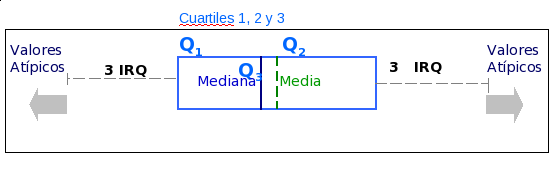
\includegraphics[scale=0.5]{images/boxplot}\\
\textbf{OJO:} el dibujo esta malo, Q1 esta al principio de la cajita, Q2 esta en la posicion de la mediana y Q3 esta al final de la caja.
Se entiende tambien que el IRQ de la izquierda es ``-3IRQ'' y no 3IRQ
Representacion visual para describir simultaneamente, varias caracteristicas importantes tales como:
\begin{itemize}
\item Centro
\item Dispersion
\item Asimetria de la distribucion
\item Identificar valores atipicos
\end{itemize}


\section{An\'alisis Bivariado}
\label{sec:cap3}
Como es parte de la Estadistica descriptiva, tiene como objetivo obtener informacion desde una muestra,
que permita entender o forumular hipotesis acerca del fenomeno que se estudia.

\subsection{Analisis Estratificado}
	El análisis estratificado pretende mostrar cómo cambia una variable (Y) cuando cambia otra (X)
	\begin{itemize}
		\item Se divide una muestra de acuerdo al valor de una variable que llamaremos variable estratificadora X
		\item Se estudia el comportamiento de otra variable  de interés Y (dependiente) en cada subgrupo o estrato
		\item Se da cuenta de cómo cambia el comportamiento de Y al cambiar de estrato X
		\item si la variable explicativa (X) es continua, definir categorías de valores posibles y separar la muestra de acuerdo a ellas
		\item Habiendo estratificado con algún criterio, medimos $\rightarrow$ frecuencias,tendencias(media, mediana,etc),dispersion(IQR)
		\item Habiendo estratificado y analizado el comportamiento de la variables por estrato$\rightarrow$ graficos, box-plots(por cada estrato)
		\item Una forma de medir el efecto de la variable presuntamente explicativa (X) sobre la explicada (Y) es el \emph{An\'alisis de Varianza}.
		\item \textbf{Idea:} si la variable estratificadora X explica bien la otra variable Y, Y no debiera variar mucho con un X constante.
	\end{itemize}
\subsubsection{Analisis de Varianza}
	\begin{itemize}
		\item Varianza Intra-Estratos(dentro de los grupos)$\ =\ \sum_{h=1}^{m}p_{h}\cdot V_{h}$, (frecuencia por varianza)
		\begin{itemize}
			\item ponderamos por el peso del estrato!!!
			\item Varianza no explicada por la variable estratificadora
		\end{itemize}
		\item Varianza Inter-Estratos(dentro de los grupos)$\ =\ \sum_{h=1}^{m}p_{h}\cdot(\bar{Y}_{h}-\bar{\bar{Y}})^{2}$
		\begin{itemize}
			\item media de cada grupo inducido por la variable explicativa X, $\bar{\bar{Y}}\ =\ \sum_{h=1}^{m}p_{h}\cdot\bar{Y}_{n}$
			\item media total o promedio ponderado de las medias por grupo.
		\end{itemize}
		\item Varianza Muestral Total:
		\begin{itemize}
			\item $V_{T}\ =\ \frac{1}{n}\sum_{i}(Y_{i}-\bar{Y})^2$ (Varianza Muestral Sin Estratificar)
			\item $V_{T}\ =\ \sum_{h=1}^{m}p_{h}\cdot V_{h}\ +\ \sum_{h=1}^{m}p_h(\bar{Y}_{h}-\bar{\bar{Y}})^{2}$
			\item $V_{T}\ =\ V_{intra}\ +\ V_{inter}$
		\end{itemize}
		\item Cuociente de Varianza Explicada:
		\begin{itemize}
			\item $\frac{V_{T}}{V_{inter}}$
			\item Medida de la calidad de la variable estratificadora X como variable explicativa para Y\\
			\item Para todo lo anterior necesitamos que Y sea continua, pero X puede ser continua o discreta, numérica o cualitativa.\\\\
		\end{itemize}
	\end{itemize}
	\textbf{Ejemplo:}
	Consideremos la siguiente hip\'otesis de estudio: Caminar ayuda a mantener un \'indice de grasa corporal adecuado.\\
	Para validar la hip\'otesis se tom\'o una muestra de 16 hombres, encuest\'andolos acerca del n\'umero de horas caminadas
	a la semana y midiendo su \% de grasa corporal. La muestra es la siguiente:\\
	\begin{center}
		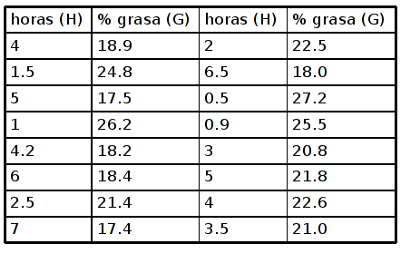
\includegraphics[height=4.5cm]{images/cap3_ej1_1}
	\end{center}
	$$\bar{G}\ =\ 21.3875$$
	$$V_{T}\ =\ 9.7898,\ Calculado\ mas\ adelante$$
	Decidimos estratificar la muestra de acuerdo al número de horas caminadas, considerando 3 clases para el conjunto de valores de esta variable:\\
	$$R\ =\ (7-0.5)\ =\ 6.5$$
	$$A\ =\ (R + 1)/3\ =\ 2.5$$
	\begin{center}
       		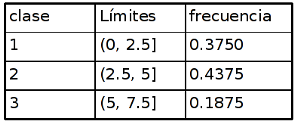
\includegraphics[height=3cm]{images/cap3_ej1_2}
       	\end{center}
	Estratificamos por cada clase de valores para la variable “horas caminadas” generandose 3 submuestras\\
	\begin{center}                                           	
       		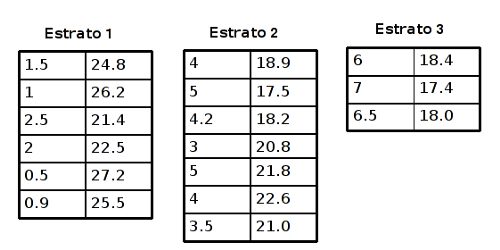
\includegraphics[height=4.5cm]{images/cap3_ej1_3}
        \end{center}
	Medimos las medias y las varianzas por estrato:\\
	\begin{center}                                           	
        	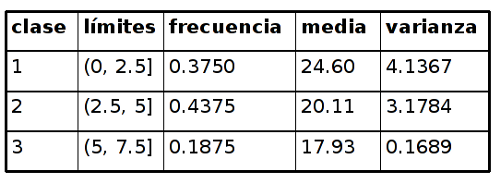
\includegraphics[height=3cm]{images/cap3_ej1_4}
        \end{center}
	Calculamos la varianza intra:
	$$V_{intra}\ =\ 0.375\cdot 4.1367\ +\ 0.4375\cdot 3.1784\ +\ 0.1875\cdot 0.1689$$
	$$V_{intra}\ =\ 2.9735$$
	Calculamos la varianza inter:
       	$$V_{inter}\ =\ 0.375\cdot (24.60\ -\ \bar{G})^2\ +\ 0.4375\cdot (20.11\ -\ \bar{G})^2\ +\ 0.1875\cdot (17.93\ -\ \bar{G})^2$$
       	$$V_{inter}\ =\ 6.8255$$
	Corroboramos la decomposicion propuesta:
	$$V_{T}\ =\ V_{intra}\ +\ V_{inter}\ =\ 2.9735\ +\ 6.8255\ =\ 9.7898$$
	$$\frac{V_{inter}}{V_{T}}\ =\ 0.6966\ \approx 70\%$$
	$$\therefore \ Hay\ una\ relacion\ bien\ significativa$$


	\emph{?`Es valida la relaci\'on entre las varianzas cuando estas se calculan normalizando la suma de cuadrados por n-1 en vez de n?}
	\begin{itemize}
		\item Cuando entremos en Estad\'istica Inferencial justificaremos porqu\'e es m\'as \'uil y correcto comparar las sumas de cuadrados
		\item $S_{T}\ =\ \sum_{I}(Y_{i}-\bar{Y})^{2}$
		\item $S_{intra}\ =\ \sum_{k=1}^{m}\sum_{i\epsilon E_{k}}(Y_{i}-\bar{Y}_{k})^2$, Suma sobre las observaciones del estraro K
		\item $S_{inter}\ =\ \sum_{k=1}^{m}(\bar{Y}_{k}-\bar{Y})^{2}$, suma sobre los estratos
	\end{itemize}
\subsubsection{Analisis de Varianza (ANOVA)}
	Comparamos la variabilidad intra versus la inter.
	\begin{itemize}
		\item $F\ =\ \frac{\frac{S_{inter}}{m-1}}{\frac{S_{intra}}{n-m}}$
		\item \emph{Estad\'istico F de Fisher (m: n\'umero de clases)}
		\item De acuerdo al valor de F podemos aseverar que la variable estratificadora induce cambios en la otra variable con una significancia estadística $\alpha$
	\end{itemize}
\subsection{An\'alisis de Contingencia o Correspondencia}
	\begin{itemize}
		\item  Dadas dos variables X, Y dividir los posibles valores de X en k grupos y los posibles valores de Y en s grupos.
		\item  Determinar luego las frecuencias conjuntas de cada par formado por uno de los grupos de X y uno de los grupos
		 para Y: con qué frecuencia las observaciones caen en un grupo X y un grupo Y simultáneamente.
		\item consta de una tabla que se realiza con las frecuencia con que en la muestra aparecen observaciones que caen en le categoria
		i de acuerdo al valor X y en la categoria j de acuerdo al valor Y
		\item \emph{Frecuencias Marginales:} (sumar todas las frecuencias y ponerlas al final de cada fila y columna)Cuando interesa la frecuencia de una de
		 las variables independiente de lo que pase con la otra  hablamos de Frecuencia Marginal de la variable X \'o Y
		\begin{itemize}
			\item $n_{i\cdot}\ =\ \sum_{j=1}^{s}n_{ij}$ Frecuencia Absoluta de la clase $A_{i}$, Frecuencias Independientes de las clases $B_{j}$
			 a la que estén asociadas: suma de los valores de la fila i-\'esima 
			\item  $n_{\cdot j}\ =\ \sum_{i=1}^{r}n_{ij}$ Frecuencia Absoluta de la clase $B_{j}$, Frecuencias Independientes de las clases $A_{i}$
			 a la que estén asociadas: suma de los valores de la columna j-\'esima 
		\end{itemize}
		\item \emph{Frecuencias Relativas Marginal:} lo mismo que la Marginal solo que cada valor se divide por el total de las muestras.
		\item \emph{Frecuencias Condicionales:} Las frecuencias condicionales de una clase $A_i$ (asociada a X) dado un grupo $B_j$
		 (asociado a Y) corresponden a la proporci\'on de casos de $B_j$ en que se observa $A_i$ y viceversa.
		\begin{itemize}
			\item $f_{i/j}\ =\ \frac{n_{ij}}{n_{\cdot j}}\ =\ \frac{f_{ij}}{f_{\cdot j}}$
			\item $f_{j/i}\ =\ \frac{n_{ij}}{n_{i\cdot}}\ =\ \frac{f_{ij}}{f_{i\cdot}}$
			\item Si se quiere condicionar a X o Y, lo que se tiene que hacer es dividir cada valor de la tabla, por la frecuencia
			 marginal de su columna(Y) o fila(X)
			\item Proporcionan una forma de medir la influencia de la variable X sobre la variable Y (o viceversa)
			\item Notar que las frecuencias se normalizan por un n\'umero m\'as reducido de casos, que corresponden a los 
			casos en que se observa el condicionante. 
		\end{itemize}
		\item \emph{Independencia}
			\begin{itemize}
				\item Diremos que X es independiente de Y si las frecuencias condicionales de X a las diferentes clases de Y son
				 todas iguales; es decir, no dependen de la clase condicionante:(y viceversa)
				$$f_{i/1}\ =\ f_{i/2}\ =\ \ldots\ =\ f_{i/s}\ \forall i$$
				$$f_{j/1}\ =\ f_{j/2}\ =\ \ldots\ =\ f_{j/r}\ \forall j$$
				\item Observaciones:
				\begin{itemize}
					\item Si X es independiente de Y: $f_{i/j}\ =\ f_{i\cdot}\ ,\forall i,j$
					\item Si Y es independiente de X: $f_{j/i}\ =\ f_{\cdot j}\ ,\forall i,j$
					\item Si X es independiente de Y: $f_{ij}\ =\ f_{i\cdot}\ \cdot\ f_{\cdot j}$
					 $$Dem:\ f_{i/j}\ =\ \frac{n_{ij}}{n_{\cdot j}}\ =\ \frac{f_{ij}}{f_{\cdot j}}\ \rightarrow f_{ij}\ =\ 
					f_{i/j}\cdot f_{\cdot j}\ =\ f_{i\cdot}\cdot f_{\cdot j},\ \forall i,j$$
					\item Si X es independiente de Y entonces Y es independiente de X: 
					$$f_{j/i}\ =\ \frac{f_{ij}}{f_{i\cdot}}\ =\ \frac{f_{ij}}{\frac{f_{ij}}{f_{\cdot j}}}$$
				\end{itemize}
				\item \emph{Informaci\'on Mutua:} 
				\begin{itemize}
					\item Si aceptamos la tabla de contingencia como una distribuci\'on aproximada podemos
					 computar la información mutua de X e Y.
					\item  Si X es independiente de Y, I=0 y  Si X = Y, I es equivalente a la entropía de X
					\item $I(x,y)\ =\ \sum_{i,j}f_{ij}\log\left(\frac{f_{ij}}{f_{i\cdot}\cdot f_{\cdot j}}\right)$
				\end{itemize}
			\end{itemize}
	\end{itemize}


\section{Correlaci\'on y Regresi\'on Lineal}
\label{sec:cap4}
%Estad\'istica Descriptiva: Correlaci\'on y Regresi\'on Lineal
\begin{itemize}
	\item Objetivo: Obtener informaci\'on desde una muestra, que permita entender o formular hip\'otesis acerca del fen\'omeno que se estudia.
	\item Tipos de An\'alisis
	\begin{itemize}
		\item Describir c\'omo se comporta una variable
		\item Describir c\'omo una variable afecta el comportamiento de a otra
		\item Describir c\'omo interaccionan varias variables
	\end{itemize}
	\subsection{An\'alisis Bivariado}
		\subsubsection{Correlaci\'on}
		Medida cuantitativa del grado de asociaci\'on entre dos variables X e Y continuas
		\begin{itemize}
			\item Covarianza: Medici\'on de los cambios con respecto al nivel medio de cada variable.\\
					 La medida depende de las magnitudes absolutas de x e y, por lo que una mayor covarianza no significa mayor asociaci\'on.\\
					 $$ cov(x,y)\ =\ \frac{1}{n}\sum_{i=1}^{n}\ (x_i\ -\ \bar{x})(y_i\ -\ \bar{y}) $$
			\item Coeficiente de Correlaci\'on de Pearson: Normaliza la covarianza con una medida de dispersi\'on para X y para Y. Es acotada entre -1 y 1.
					 $$\rho_{xy}\ =\ \frac{cov(x,y)}{\sigma_x\sigma_y}$$


			\begin{itemize}
				\item Observaciones
				\begin{itemize}
					\item Si x e y tienen una relaci\'on lineal exacta, la correlaci\'on de Pearson es igual al signo de la pendiente.
					\item $cov(x,y)\ =\ a\cdot var(x)$ 
					\item $var(y)=\ a^2\cdot var(x)$ 
					\item Una correlaci\'on nula indica que no hay relaci\'on aparente entre las variables (penditene 0). 
				\end{itemize}
				\item Correlaci\'on y Ruido\\
					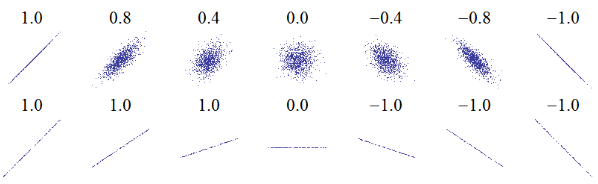
\includegraphics[height=3.5cm]{images/ruido}
				\item Limitaciones: Para un mismo valor del coeficiente pearson...\\
					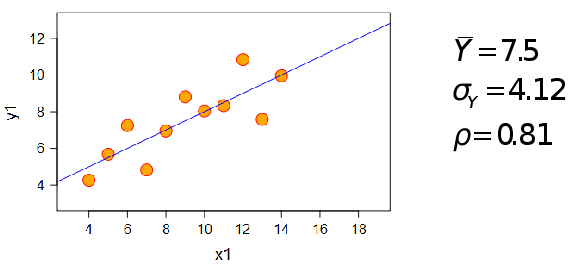
\includegraphics[height=3.5cm]{images/cap4-limit_pearson1.png}\\
					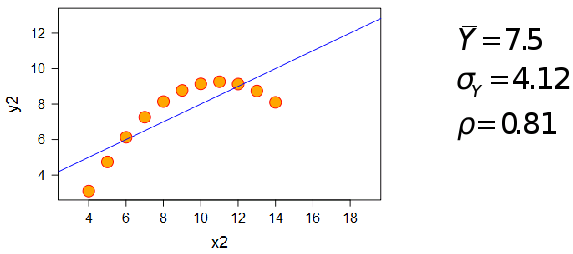
\includegraphics[height=3.5cm]{images/cap4-limit_pearson2.png}\\
					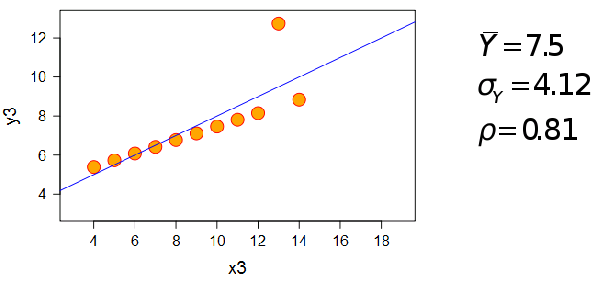
\includegraphics[height=3.5cm]{images/cap4-limit_pearson3.png}\\
					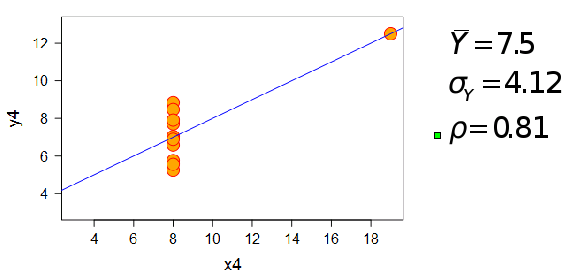
\includegraphics[height=3.5cm]{images/cap4-limit_pearson4.png}
			\end{itemize}
		\end{itemize}
		\subsubsection{Regresi\'on}
			Modelo de una variable y (dependiente) como funci\'on de otra x (independiente).\\
			$$Y\ =\ f(X)+\varepsilon$$
		\begin{itemize}
			\item Regresi\'on Lineal: Ajustar el modelo lineal consiste en buscar par\'ametros b0 y b1 que hagan el modelo adecuado.
				$$f(x)\ =\ b_1x\ +\ b_0$$
			\begin{itemize}
				\item Estimando los coeficientes: Minimizar error cuadr\'atico\\
					$$I^2(x,y)\ =\ (y-f(x))^2$$
					$$I^2(x,y)\ =\ (y-b_1x-b_0)^2\ = \varepsilon^2$$\\
					Ahora buscamos minimizar el error promedio:\\
					$$R_s\ =\ \sum_{x_i\ \epsilon\ S}(y_i-b_1x_i-b_0)^2$$
					$$R_s\ =\ \sum_{x_i\ \epsilon\ S}I^2(x_i,y_i)$$
					Y despues de analizar las derivadas en funci\'on de $b_0$, $b_1$ y ver unos cuantos determinantes..
					$$b_1\ =\ \frac{cov(x,y)}{var(x)}$$
					$$b_0\ =\ \bar{y}\ -\ \frac{cov(x,y)}{var(x)}\bar{x}$$
				\item An\'alisis de la Varianza: Sirve para ver que tan bueno es nuestro modelo descriptivo.\\
				\begin{itemize}
					\item Variabilidad explicada por el modelo: $$S(\hat{y})\ =\ \sum_{i}(\hat{y_i}\ -\ \bar{\hat{y_i}})^2\ =\ \sum_{i}(\hat{y_i}\ -\ \bar{y_i})^2$$
					\item Variabilidad NO explicada por el modelo:$$R_S\ =\ \sum_{i}\varepsilon_{i}^{2}\ =\ \sum_{i}(y_i\ -\ \hat{y})^2$$
					\item Variabilidad Total de Y:
								$$S(y)\ =\ \sum_{i}(y_i\ -\ \bar{y})^2$$\\
								Y esto es igual a la variabilidad explicada + la no explicada:
								$$S(y)\ =\ \sum_{i}(\hat{y_i}\ -\ \bar{y_i})^2\ +\ \sum_{i}(y_i\ -\ \hat{y})^2 $$
				\end{itemize}
				\item Coeficiente de Determinaci\'on: Fracci\'on de la variabilidad que s\'i es explicada por el modelo lineal (\% de ajuste):
					$$D\ =\ \frac{S(\hat{y})}{S(y)}$$\\
					Y ahora si sabemos que:
					$$S(\hat{y})\ =\ \sum_{i}(\hat{y_i}-\bar{\hat{y_i}})^2\ =\ \sum_{i}(\hat{b_0}\ +\ \hat{b_1}x_i \ -\ \bar{y})^2$$
					$$S(\hat{y})\ =\ \sum_{i}(\ \hat{b_1}x_i \ +\ \hat{b_1}\bar{x})^2$$
					$$S(\hat{y})\ =\ \hat{b_1^2}\cdot n\cdot var(x)$$\\
					El coeficiente nos queda:
					$$D\ =\ \frac{\hat{b_1^2)}\cdot n\cdot var(x)}{n\cdot var(y)}$$
					$$D\ =\ \frac{\hat{b_1^2)}\cdot var(x)}{var(y)}$$\\
					Y por \'ultimo, reemplazando el b:
					$$D\ =\ \rho_{xy}^2$$
					$$\therefore\ D\ =\ \frac{cov^2(x,y)}{var(x)\ var(y)}$$
			\end{itemize}
			\item Regresiones con trasnformaci\'ones lineales: Uno construye un modelo lineal en una variable independiente auxiliar.
				$$Y\ =\ b_0\ +\ b_1ln(X)\ +\ \varepsilon$$
				$$Z\ =\ X^2$$
	\end{itemize}
\end{itemize}


\section{Inferencia Estadistica}
\label{sec:cap5}
\subsection{Probabilidad: Axiomas y Modelos}
Metodos para recolectar y analizar datos acerca de un fenomeno acerca del cual se tiene \textbf{intertudumbre}. Obtener conclusiones:
\begin{itemize}
\item Entender un fenomeno
\item Tomar decisiones
\item Controlar un fenomeno
\end{itemize}

\subsection{Metodo estadistico}
\begin{itemize}
\item Recolectar datos
\item Analizar los datos
\item Modelar el fenomeno
\item Sacar conclusiones
\end{itemize}

\subsubsection{Probabilidades}
Modelo matematico para la incertidumbre. Nocion Frecuentista generaliza la idea de frecuencia de un suceso o resultado

\subsubsection{Espacio Muestral $\Omega$}
Conjunto de resultados elementales posibles.\\
Ej. Tirar un dado dos veces.\\
$\Omega = {(1,1) (1,2) (1,3) \ldots (6,6)}$\\
Ej. Tiempo de espera en una cola de supermercado.\\
$\Omega = [0,100]$\\
\subsubsection{Eventos}
Cualquier subconjunto del espacio muestral $\Omega$ se denomina \textbf{evento}. Se busca hablar de la \textbf{probabilidad de eventos}
\subsubsection{Axiomas}
Una medida de probabilidad es una medida de la certeza de un evento. La probabilidad de un evento que debiera reflejar la certeza con que obtendremos uno de los resultados del evento.
\begin{itemize}
\item Axioma 1: $P(\Omega) = 1$
\item Axioma 2: $P(A) >= 0$
\item Axioma 3: Si A y B son eventos disjuntos P(A U B) = P(A) + P(B)
\end{itemize}
\subsubsection{Implicancia de los Axiomas}
\begin{itemize}
\item $P(A^c) = 1 - P(A)$
\item Si A $\subset$ B $\rightarrow P(A) <= P(B)$
\item P(B-A) = P(B) - P(A $\bigcap$ B)
\item P(A $\bigcup$ B) = P(B) + P(B) - P(A $\bigcap$ B)
\item $P(\bigcup A_i) <= \sum P(A_i)$
\end{itemize}

\subsubsection{Sigma Algebra}
Coleccion de eventos que son posible \textbf{medir}. Debe satisfacer propiedades minimas de cerradura para que sea util. Como se trata de subconjuntos, tiene sentido hablar de operaciones como complementos, intersecciones, uniones, diferencias.\\
Dado un espacio muestral $\Omega$, una sigma algebra es una coleccion C de sobconjuntos de $\Omega$ tal que:
\begin{itemize}
\item C $\neq \Phi$
\item Si A $\epsilon$ C entonces $(\Omega - A) \epsilon C$
\item Si $A_1 \ldots A_n \epsilon C => A_1 U \ldots U A_ni\ \epsilon\ C$ 
\end{itemize}

\subsubsection{Medida de Probabilidad}
Dado un conjunto $\Omega$ y una sigma algebra C, una medida de probabilidad es una funcion que:\\
$P: C \rightarrow R$

\begin{itemize}
\item $P(\Omega) = 1$
\item $P(A) >= 0$ para todo A $\epsilon$ C
\item Si $A_1 \ldots A_n \epsilon C$ son disjuntos, $P(A_1 \ldots \bigcup A_n) = P(A_1) + \ldots + P(A_n)$
\end{itemize}
$(\Omega, C, P)$: Espacio de Probabilidad\\
$(\Omega, C)$: Espacio Medible\\
C es la Familia de los Eventos Medibles\\
Podemos pensar como probabilidad la frecuencia con que se ve un resultado si observamos el fenomeno multiples veces.

\subsubsection{Nocion frecuentista}
Suponer repetir un experimento N veces y de estas, $N_a$ veces observamos un resultado contenido en el evento A. La probabilidad seria:\\ \\
$P(A) = lim_{n \rightarrow \infty} \frac{N_a}{N}$

\subsubsection{Nocion te\'orica}
Si tenemos un experimento que puede ocurrir de N formas, nuestro espacio muestral es finito $\Omega$.\\
Una sigma algebra posible es Pow($\Omega$).\\
Una medida de probabilidad \textbf{natural} es:\\ \\
$P(A) = \frac{|A|}{N} = \frac{|A|}{\Omega}$ donde $|A|$ es la cardinalidad de A.\\
$(\Omega, Pow(\Omega), P)$ es un espacio de probabilidad valido.\\ \\
Ej. Tirar un dado y que salga par:\\
$P({2,4,6}) = \frac{|{2,4,6,}|}{|{1,2,3,4,5,6,}|} = \frac{3}{6} = \frac{1}{2} = \frac{ResultadosFavorablesAlEventoA}{ResultadosPosibles}$

\subsubsubsection{Combinaciones}
Formas distintas de obtener r elementos de un lote de n:\\
$C(n,r) = \frac{n!}{n!(n-r)!}$

\subsection{Nocion Bayesiana}
``La probabilidad de que el cafe este frio es 0.8''\\
Es valido querer aclarar nuestro grado de incertidumbre. ?`Podr\'iamos darle una interpretaci\'on a la sentencia bajo la nocion frecuentista o teorica?.\\
La Nocion Bayesiana se entiende como la probabilidad con un grado subjetivo de certeza. Lo importante es desarrollar una forma de operar con estos \textbf{grados de certeza} para combinarlos y actualizarlos si se tienen nuevas observaciones. Es compatible con la teorica o frecuentista.




\section{Probabilidad Condicional}
\label{sec:cap6}
\textbf{Ejemplo:} ?`Cu\'al es la ``probabilidad'' de que tardemos m\'as de 30 minutos en la cola del almuerzo? si sabemos que son las
13:15 de la tarde?
\begin{center}
	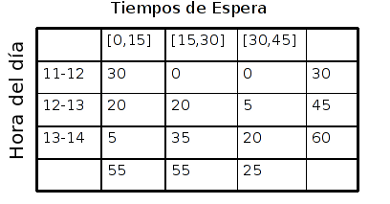
\includegraphics[height=3cm]{images/cap6_ej1_1}
\end{center}
Entonces claramente es $\frac{20}{25+55+55}\ \approx\ 14.81\%$
\subsection{Probabilidad Condicional}
\begin{itemize}
	\item Sean A,B dos sucesos tal que $P(B)>0$
	\item La probabilidad de A condicionada a la ocurrencia de B es:
	$$P(A|B)\ =\ \frac{P(A\cap B)}{P(B)}$$
	\item Notemos que la idea de frecuencias coindicionales calza perfectamente en este modelo
	\item Centra el foco de atencion en el hecho que se sabe que ha ocurrido el evento B
	\item Estamos indicando que el espacio muestral de interes se ha ``reducido'' solo a
	aquellos resultados que definen la ocurrencia del evento B
	\item Entonces $P(A|B)$ ``mide'' la probabilidad relativa de A con respecto al espacio
	reducido B
\end{itemize}
\subsection{Se respetan los axiomas basicos}
\begin{itemize}
	\item $P(A|B)\ \geq\ 0$
	\item $P(\Omega|B)\ =\ 1$
	\item Sean $A_{1},A_{2},\ldots,A_{n}$ disjuntos $A_{i}\cap A_{j}\ =\ \emptyset\ \forall i\neq j$
	$$P(\cup A_{i}|B)\ =\ \sum P(A_{i}|B)$$
\end{itemize}
\textbf{Ejemplo2:} Si lanzamos dos dados (4 caras) ?`Cu\'al es la probabilidad de que el m\'aximo
	de los resultados sea par dado que el m\'inimo de los resultados es 3?\\
	$$\Omega\ =\ {(1.1),(1.2),(1.3),\ldots,(4.4)}$$
	donde la minima es 3 $B\ =\ {(3.3),(3.4),(4.3)}$\\
	donde el maximo es par $A\ =\ {(3.4),(4.3)}$\\
	$$P(A|B)\ =\ \frac{2}{3}\ \Longleftrightarrow \frac{P(A\cap B)}{P(B)}\ =\ \frac{\frac{2}{16}}{\frac{3}{16}}\ =\ \frac{2}{3}$$
\textbf{Ejemplo3:} En una encuesta se ha determinado que los fines de semana el 45\% de la poblacion
	lee la tercera, el 35\% lee el mercurio y el 5\% lee ambos diarios. ?`Cu\'al es la probabilidad
	de que un lector de la tercera lea tambi\'en el mercurio?\\
	$$\frac{P(A\cap B)}{P(B)}\ =\ \frac{\frac{5}{100}}{\frac{45}{100}}\ =\ \frac{1}{9}$$
\textbf{Ejemplo4:} En una f\'abrica se ha recopilado la siguiente informaci\'on (expresar como probabilidades)
	\begin{itemize}
		\item El 25\% de las piezas con fallas superficiales son funcionalmente defectuosas
		\item Se sabe que el 10\% de las piezas manufacturadas tienen fallas visibles
		en la superficie
		\item Tambi\'en se ha encontrado que el 5\% de las piezas que no tenian fallas
		superficiales son funcionalmente defectuosas
	\end{itemize}
	\begin{center}
		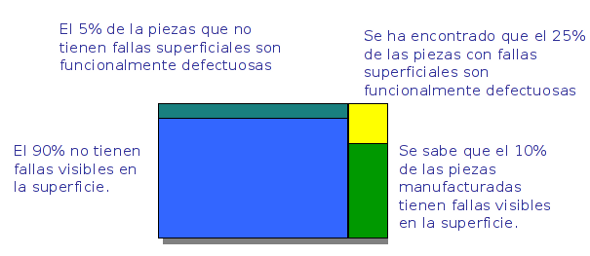
\includegraphics[height=4cm]{images/cap6_ej4_1}
	\end{center}
	B = \{ Pieza funcionalmente defectuosa \}\\
	A = \{ Pieza tiene una falla visible en la superficie \}\\
	$P(B|A)\ =\ 25\%$\\
	$P(A)\ =\ 10\%$\\
	$P(B|A^{c})\ =\ 5\%$\\
	$P(A^{c})\ =\ 90\%$\\
	$P(B)\ =\ P(B|A)P(A)\ +\ P(B|A^{c})P(A^{c})\ =\ \frac{25}{100}\cdot \frac{10}{100}\ +\ \frac{5}{100}\cdot \frac{90}{100}\ =\ \frac{7}{100}$\\
	$P(A\cap B)\ =\ P(B\cap A)\ =\ \frac{P(B|A)}{P(A)}\ =\ \frac{25}{1000}\ =\ \frac{1}{40}$\\
	$$P(A|B)\ =\ \frac{P(A\cap B)}{P(B)}\ =\ \frac{\frac{1}{40}}{\frac{7}{100}}\ =\ \frac{5}{14}$$
\subsection{Distintos Casos de la Probabilidad Condicional}
	\begin{center}
		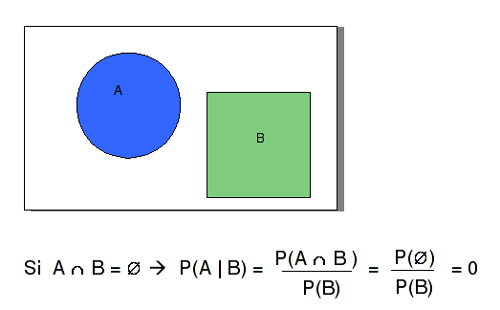
\includegraphics[height=4cm]{images/cap6_1}\\
		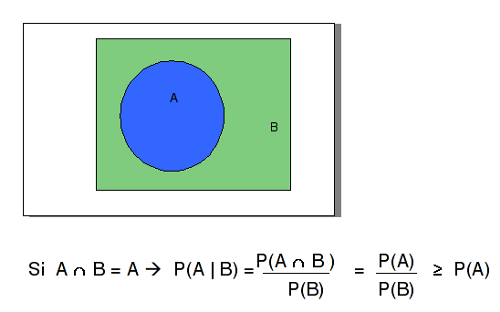
\includegraphics[height=4cm]{images/cap6_2}\\
		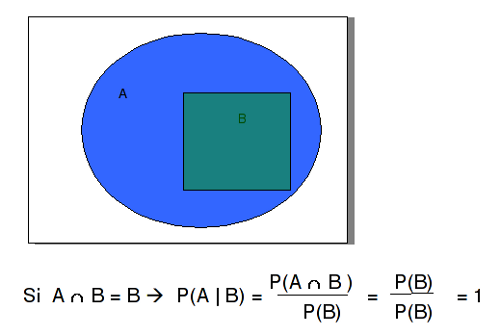
\includegraphics[height=4cm]{images/cap6_3}\\
		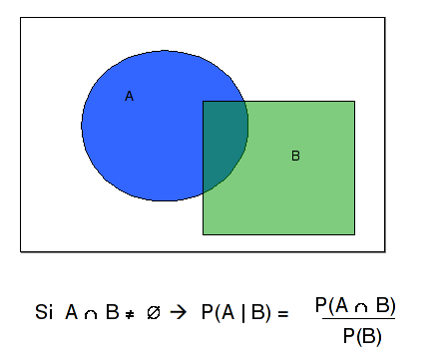
\includegraphics[height=4cm]{images/cap6_4}
	\end{center}
\subsection{Probabilidad Marginal}
	Si estudiamos la relación entre una serie de eventos $A,B,C$, llamaremos ``probabilidades
	marginales'' a las probabilidades no condicionales $P(A),\ P(B)\ y\ P(C)$. 
\subsection{Regla de Bayes}
	\begin{itemize}
		\item Sean A, B dos sucesos tal que $P(A)$, $P(B)>0$.
		\item Establece una relacion entre las probabilidades condicionales $P(A|B)$ y $P(B|A)$
		$$P(A|B)\ =\ \frac{P(B|A)P(A)}{P(B)}$$
		\item Se sigue inmediatamente de la definicion de probabilidad condicional
	\end{itemize}
\subsection{Probabilidad Total}
	Sean B1, B2,....,Bn  eventos mutuamente excluyentes tal que su uni\'on conforma
	el espacio muestral:
	$$P(\bigcup_{i=1}^{n}B_{i})\ =\ 1$$
	Entonces:
	$$P(A)\ =\ P(A|B_{1})P(B_{1})\ +\ \ldots\ +\ P(A|B_{n})P(B_{n})$$
	\begin{center}
		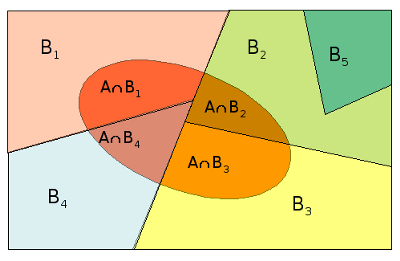
\includegraphics[height=4cm]{images/cap6_5}\\
	\end{center}
	\textbf{Ejemplo5:} Un producto se fabrica en 5 plantas que producen el 20\%, 25\%, 30\%,
	 15\% y 10\% respectivamente. Las probabilidades de fallas en cada planta est\'an dadas
	por: 0.2, 0.1, 0.15, 0.3, 0.0 ?`Cu\'al es la probabilidad de que un producto venga fallado?\\
	$P(B_1)\ =\ 20\%$\\
	$P(B_2)\ =\ 25\%$\\
	$P(B_3)\ =\ 30\%$\\
	$P(B_4)\ =\ 15\%$\\
	$P(B_5)\ =\ 10\%$\\
	$P(A)\ =\ P(A|B_{1})P(B_1)\ +\ \ldots\ +\ P(A|B_5)P(B_5)$\\
	$$P(A)\ =\ 0.2\cdot \frac{20}{100}\ +\ \ldots\ +\ 0.0\cdot \frac{10}{100}\ =\ \frac{15.5}{100}\ =\ 15.5\%$$
	\textbf{Ejemplo6:} Continuando con el anterior...supongamos de que se elige aleatoriamente
	un producto y se encuentra que est\'a fallado. ?`Cu\'al es la probabilidad que sea
	manufacturado en Planta $B_3$?\\
	$$P(B_{3}|A)\ =\ \frac{P(A|B_{3})P(B_{3})}{P(A)}\ =\ \frac{0.15\cdot \frac{30}{100}}{0.155}\ =\ 0.29\ =\ 29\%$$
\subsection{Independencia}
	\begin{itemize}
		\item Dos eventos A y B se dicen independientes ssi:
		$$P(A\cap B)\ =\ P(A)P(B) \rightarrow\ P(A|B)\ =\ P(A)\ y\ P(B|A)\ =\ P(B)$$
		\item Sean ${A_{i}:i\epsilon I={1,2,3,\ldots,k}}$ una colecci\'on de eventos de
		 $(\Omega,\xi,P)$. Se dice que los elementos son conjuntamente independientes 
		 para todo subconjunto de indices $J$:
		$$P(\bigcap_{j\epsilon J}A_{j})\ =\ \prod_{j\epsilon J}P(A_{i})$$
	\end{itemize}
	\textbf{Ejemplo7:} Sea $(\Omega,2^{\Omega},P)$ modelo de probabilidad.
		$$\Omega\ =\ {(1,0,0),(0,1,0),(0,0,1),(1,1,1)}$$
		$$P({w_{i}})\ =\ \frac{1}{4}$$
		Sean $A_{1},\ A_{2},\ A_{3}$ eventos de $(\Omega,2^{\Omega},P)$:\\
		\begin{itemize}
			\item $A_{1}:$ Primera coordenada es 1
			\item $A_{2}:$ Segunda coordenada es 1
			\item $A_{3}:$ Tercera coordenada es 1
		\end{itemize}
		$P(A_{1})\ =\ \frac{1}{2}$\\
		$P(A_{2})\ =\ \frac{1}{2}$\\
		$P(A_{3})\ =\ \frac{1}{2}$\\
		$P(A_{1}\cap A_{2})\ =\ \frac{1}{4}\ =\ P(A_{1})P(A_{2})$\\			
		$P(A_{1}\cap A_{3})\ =\ \frac{1}{4}\ =\ P(A_{1})P(A_{3})$\\			
		$P(A_{2}\cap A_{3})\ =\ \frac{1}{4}\ =\ P(A_{2})P(A_{3})$\\
		Todos son independientes (Independencia de a Pares)\\
		$P(A_{1}\cap A_{2}\cap A_{3})\ =\ \frac{1}{4}\ \neq\ P(A_{1})P(A_{2})P(A_{3})$\\
		No son independientes como Familia\\


%\section{Variables Aleatorias y Distribuciones}
%\label{sec:cap7}
%	Idea Intuitiva: variable que toma valores con determinada ``regla de probabilidad''.\\
	Nos interesa hacer una descripci\'on matem\'atica de fen\'omenos no deterministas (inciertos). Por lo que necesitamos entonces mediciones cuantitativas.\\
	Una variable aleatoria toma valores en los\'umeros reales.

	\subsection{Variables Aleatorias}
		\begin{itemize}
			\item Mapeo de Resultados:\\
				Como una idea m\'as formal, usaremos variables aleatorias X para mapear resultados de un espacio muestral a n\'umeros reales $X: \Omega \leftarrow R$.\\
				No siempre se mapean resultados elementales a n\'umeros. Muchas veces se mapean eventos no at\'omicos a un mismo n\'umero.\\
				En general, nos interesar\'a ser\'a determinar la ``ley de probabilidad'' que rige el comportamiento de la variable aleatoria que estamos estudiando: con qu\'e probabilidad observamos ciertos valores.
			\item Definici\'on:
                             Sea $(\Omega,\ C,\ P)$ un espacio de probabilidad y $(R,\ \beta)$ un espacio de medida definido sobre los reales $(R)$. Una variable aleatoria se define como una funci\'on $X: \Omega \leftarrow R$ tal que para todo $B$ en $\beta$, su pre-imagen $X^{-1}(B)$ est\'a en $C$.
			\item Requerimientos de la Colecci\'on de eventos medibles:
			\begin{enumerate}
				\item no vac\'ia
				\item cerrada bajo complementos
				\item cerrada bajo uniones numerables
			\end{enumerate}
			\item Sigma-\'algebra de Borel ($\beta$):\\
				Queremos poder medir la probabilidad de que la variable aleatoria tome valores en intervalos [a, b].\\
				Incluimos primero todos los intervalos de la forma $(-\infty, x]$ con x en R.\\
  				Cerramos finalmente la familia bajo complementos y uniones numerables.
			\item Probabilidad Inducida: La propiedad que le pedimos a las variable aleatorias permite medir probabilidades en R.\\
				Para todo $B$ en la sigma-\'algebra $\beta$: $$P(B)\ :=\ P(w\ :\ X(w)\ esta\ en\ B)\ =\ P(X^{-1}(b))$$ \\
				S\'olo gracias a que $X^{-1}(b)$ es medible en el espacio de probabilidad original podemos calcular esta probabilidad!
		\end{itemize}
	\subsection{Funci\'on de Distribuci\'on}
		\begin{itemize}
			\item Definici\'on:\\
                         	La distribuci\'on asociada a una variable aleatoria X se define como la funci\'on F: R \-> [0,1] $$ F(x)\ =\ P((-\infty, x])$$
			\item M\'etodo:\\
				Existen dos metodos, el facil y poco-practico:
				\begin{enumerate}
					\item Determinar el subconjunto de valores de $\Omega$ mapeados a esos valores de R.
					\item Calcular la probabilidad de ese conjunto de valores de $\Omega$.
				\end{enumerate}
				Y el que si hay que seguir, en el cual la idea es caracterizar la probabilidad de los eventos que generan la sigma \'algebra en $R: (-\infty, x]$.\\
				Descomponemos en eventos para los que conocemos la probabilidad:
				$$(-4,5]\ =\ (-\infty,\ 5] - (-\infty,\ 4]$$
				$$P(-4,5]\ =\ P(-\infty,\ 5] - P(-\infty,\ 4]$$
				$$P(-4,5]\ =\ F(5)\ -\ F(4)$$

			\item Variables Discretas:
				En este caso, existen ``intervalos de probabilidad'' para cada punto, describiendo saltos por cada $X=x_n$.\\
					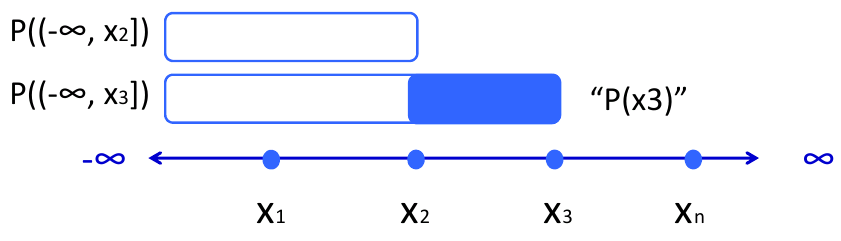
\includegraphics[height=3.5cm]{images/cap7-discretas.png}\\
				$$\therefore\ P(X=x_n)\ =\ F(x_n)\ -\ F(x_{n-1})$$
			\item Variables Continuas: No podemos ver el problema por intervalos definidos, ya que cada itervalo posee infinitos puntos. Se utiliza el concepto de densidad de Probabilidad.
				
		\end{itemize}
	\subsection{Funci\'on de Probabilidad o Cuant\'ia}
		\begin{itemize}
			\item Definici\'on
                           La funci\'on de probabilidad o cuant\'ia asociada a una variable aleatoria discreta se define como la funci\'on $p: S* \leftarrow [0,1]$ 
				$$p(x_0)\ =\ p(-\infty)$$
				$$p(x_n)\ =\ F(x_n)\ -\ F(x_n-1)$$\\
				 S es el conjunto de valores que toma X (soporte de la distribuci\'on).

			\item M\'etodo: Para calcular la probabilidad de cualquier evento A medible en R.
				$$P(A)\ =\ \int_{A}p(x_i)dx\ =\ \sum_{x_i\ \varepsilon\ A}p(x_i)$$
			\item Propiedades que se deben cumplir
				$$1\ =\ P(R)\ =\ \sum_{x_i\ \varepsilon\ R}p(x_i)$$
				$$1\ =\ \sum_{i}^{n}p(x_i)$$
			\item Densidad de Probabilidad (para variables continuas)\\
				Si existe una funci\'on p(x) tal que para todo evento A en los reales, se verifica:
				$$P(A)\ =\ \int_{A}p(x)dx$$\\
				En donde $p(x)$ se denomina funci\'on de densidad de probabilidad y X se dice absolutamente continua.
				\begin{itemize}
					\item Probabilidad de un evento en particular:
						$$F(x)\ =\ \int_{-\infty}^{x}p(x)dx$$
				\end{itemize}

		\end{itemize}


%\section{Momentos y Funci\'on Generadora}
%\label{sec:cap8}
%\subsection{Variables Aleatorias}
	\subsubsection{\bf Tendencia de la variable.}
	\subsubsubsection{Esperanza}
	Definicion: La esperanza o valor esperado de una variable aleatoria X se define como.
	$$ E(X) = \sum_{i=1}^n x_i \cdotp p(x_i) ,\ caso\ discreto$$
	$$ E(X) = \int_{- \infty}^{\infty} x \cdotp p(x) ,\ caso\ continuo$$
	En general, el valor esperado de una funci\'on g(X) de la variable aleatoria estar\'a dado por:
	$$ E(g(X)) = \int_{- \infty}^{\infty} g(x)p(x) ,\ caso\ discreto $$
	$$ E(g(X)) = \sum_{i=1}^{n} g(x_i)p(x_i) ,\ caso\ continuo $$
	Notemos que la esperanza es un operador lineal:
	$$ E(a \cdotp g(x) + b \cdotp h(x)) = a \cdotp E(g(x)) + b \cdotp E(h(x))$$
	\subsubsubsection{Mediana}
	Definicion: La mediana de una variable aleatoria discreta X se define como el valor $ x_0.5 $ tal que
	$$ \sum_{x_i < x_{0.5}} p(x_i) < 0.5 $$
	$$ \sum_{x_i \ge x_{0.5}} p(x_i) \ge 0.5 $$
	Definicion: La mediana de una variable aleatoria continua X se define como
	$$ x_{0.5} = F^{-1}(0.5)$$
	Es decir
	$$ \int_{- \infty}^{x_{0.5}} p(x) = 0.5 $$
	\subsubsubsection{Percentiles Arbitrarios}
	Definicion: El percentil de orden q asociado a una variable aleatoria continua se define como el valor $ x_q $ que satisface
	$$ \sum_{x_i < x_q} p(x_i) < q  $$
	$$ \sum_{x_i \ge x_q} p(x_i) \ge q $$
	Con $ 0 \le q \le 1 $ .\\
	Definicion: El percentil de orden q asociado a una variable aleatoria continua se define como
	$$ x_q = F^{-1}(q) $$
	Con $ 0 \le q \le 1 $ .\\
	\subsubsubsection{Moda}
	Definicion: Un valor m se dice una moda o valor modal de una variable aleatoria discreta X si
	$$ m = arg\ max_{i}\ p(x_i)  $$
	Definicion: UN valor m se dice una moda o valor modal de una variable aleatoria continua X si
	$$ \frac{\partial f}{dx} \mid_{x=m} = 0  $$
	\subsubsection{\bf Dispersi\'on al rededor de su tendencia.}
	\subsubsubsection{Varianza}
		Definicion: La varianza de una variable aleatoria X se define como 
		$$ Var(X) = E((X - E(X))^2)  $$
		\begin{itemize}
			\item Caso Discreto
				$$ Var(X) = \sum_{i=1}^{n} (x_i - E(X))^2 p(x_i) $$
			\item Caso Continuo
				$$ Var(X) = \int_{- \infty}^{\infty} (x - E(X))^2 p(x)dx  $$
		\end{itemize}
	\subsubsubsection{Desviaci\'on Est\'andar}
		Definicion: La desviaci\'on estandar de una variable aleatoria X se define como
		$$ \sigma = \sqrt{Var(X)}  $$
	\subsubsubsection{Rango Inter-Cuart\'ilico}
		Definicion: El rango inter-cuartilico asociado a una variable aleatoria se define como
		$$ IQR = x_{3/4} - x_{3/4}  $$
		O sea, la diferencia entre percentiles 0.75 y 0.25.
	
	\subsubsection{Momentos}
		Son las medidas descriptivas que caracterizan la distribucion de probabilidad de una variable aleatoria.\\
		\\ {\bf Idea}
		\begin{itemize}
		\item Generar medidas descriptivas que caractericen la distribucion de probabilidad de una variable aleatoria.
		\item Usar potencias de la variable aleatoria, tal como los monomios de una expansion de Taylor.
		\end{itemize}
		Definicion: El k-\'esimo momento de una variable aleatoria X se define como
		$$ \mu_{k}^0 = E(X^k),\ \ \ k \epsilon N  $$
		Nota: La esperanza es el primer momento :O .
	\subsubsection{Momentos Centrales}
		Definicion: El k-\'esimo momento central de una variable aleatoria X se define como
		$$ \mu_k = E((X - E(X))^k),\ \ \ k \epsilon N  $$
		Nota: La varianza es el segundo momento central. El primer momento central es nulo :O.\\
	\subsubsection{Funcion generadora de Momentos}
		Definicion: La funcion generadora de momentso (fgm) asociada a una variable aleatoria X se define como
		$$ m_x : R \rightarrow R  $$
		$$ m_x(t) = E(exp(t \cdotp X))  $$
		\begin{itemize}
			\item Caso Discreto
			$$ m_x(t) = \sum_{i=1}^n exp(t \cdotp x_i)p(x_i)  $$
			\item Caso Continuo
			$$ m_x(t) = \int_{-\infty}^{\infty} exp(t \cdotp x)p(x)dx  $$
		\end{itemize}
		Proposicion: El l-esimo momento de la fgm de una variable aleatoria X esta dado por
		$$ \mu_{k}^0 = \frac{dm_x(t)}{dt} \mid_{t=0}  $$



\end{document}
